\section{Esercizio 7}

\vfill

Si generino due classi di eventi. La prima classe chiamata \textsl{segnale} con distribuzione gaussiana bidimensionale centrata in $(x,y) = (4,4)$ e parametri $\sigma_x=\sigma_y=1$, $\rho=0$; la seconda chiamata \textsl{fondo} con distribuzione normale bidimensionale centrata in $(x,y) = (0,1)$ e parametri $\sigma_x=\sigma_y=1.5$, $\rho=0.7$. Si utilizzi uno dei metodi MVA illustrati a lezione per separare le due classi di eventi e si caratterizzi il risultato in termini di purezza del segnale e rigezione del fondo.

\vfill
\vfill

\[* * * \] 

\vfill
\vfill

\noindent In generale, considerate due classi di eventi multivariati $\vec{x}_0 ,\,\vec{x}_1 \in \mathbb{R}^n$ corrispondenti alle rispettive ipotesi $H_0$: "Evento da attribuire al fondo" e $H_1$: "Evento da attribuire al segnale", si può pensare di definire dei test d'ipotesi in grado di attribuire ogni singolo evento a una classe o all'altra, lavorando su una variabile scalare opportunamente costruita a partire da $\vec{x}_0 $ e $\vec{x}_1$. In tal modo da un lato si riduce convenientemente la dimensionalità del problema (rispetto al definire un \emph{decision boundary} $n-1$ dimensionale) e allo stesso tempo, se facciamo in modo di combinare additivamente le differenze tra $H_0$ e $H_1$, si massimizza l'efficacia del test d'ipotesi.\\

\vfill
\vfill

\noindent Dal momento che nel nostro caso trattiamo due distribuzioni gaussiane con media diversa possiamo semplicemente definire un  \emph{decision boundary} lineare e proiettare i dati lungo una retta perpendicolare ad esso. Su tale proiezione si effettuerà il taglio per il test d'ipotesi.\\

\vfill
\vfill

\noindent L'idea è quindi di definire uno scalare $t(\vec{x}) = \vec{a}\cdot\vec{x}$, dove il parametro $\vec{a} \in \mathbb{R}^n$ sia scelto in modo che la separazione tra le distribuzioni teoriche $g(t|H_0)$ e $g(t|H_1)$ sia massima. Per fare questo si massimizza la quantità

\smallskip

\begin{equation*}
J(\vec{a}) = \frac{(\tau_{_1} - \tau_{_0})^2}{\sigma_{_0}^2 + \sigma_{_1}^2},
\end{equation*}

\smallskip

\noindent dove $\tau_{_0}$ e $\tau_{_1}$ indicano i valori medi della variabile $t$ rispettivamente per fondo e segnale e similmente le $\sigma_{_0}^2,\,\sigma_{_1}^2$ ne rappresentano le varianze. La $J(\vec{a})$ rappresenta una buona misura  della "distanza" tra le due distribuzioni per $t(\vec{x})$, dal momento che rapporta il bias tra i due valori medi alla somma delle rispettive varianze.\\

\vfill

\noindent Dalla condizione $\mathop{\partial_{\vec{a}}}[J(\vec{a})] = 0$ si ottiene  $\vec{a}_\mathrm{max} \propto \mathbb{W}^{-1}(\vec{\mu}_{_1} - \vec{\mu}_{_0})$, con $\vec{\mu}_{_0}$ e $\vec{\mu}_{_1}$ valori medi rispettivamente di $\vec{x}_0$ e $\vec{x}_1$, e $\mathbb{W}$ matrice di covarianza combinata, per cui in sostanza dobbiamo proiettare i dati generati lungo la retta individuata da $\vec{a}_\mathrm{max}$ e su tale proiezione fissare un $t_\mathrm{cut}$ per il test d'ipotesi. La statistica $t(\vec{x})$ è nota come \emph{discriminante lineare di Fisher}.\\

\vfill
\vfill

\noindent L'implementazione di tale metodo sugli eventi generati risulta dunque nel calcolo delle medie campionarie $\vec{m}_i$ e della conseguente matrice di dispersione combinata $\mathbb{S}_\mathrm{w} = \mathbb{S}_0 + \mathbb{S}_1$, con $\mathbb{S}_i = \sum_{\vec{x}}(\vec{x} - \vec{m}_i)\cdot(\vec{x} - \vec{m}_i)$; quindi nella costruzione del discriminante campionario come la proiezione dei dati sul vettore

\vfill

\begin{equation*}
\vec{v} = \mathbb{S}_\mathrm{w} ^{-1}(\vec{m}_1 - \vec{m}_0).
\end{equation*}

\vfill
\vfill
\vfill
\newpage

\noindent Riportiamo di seguito il codice per la generazione di $10^3$ eventi per classe e la costruzione del relativo discriminante lineare:

\begin{lstlisting}[language=python, style=Pystyle, caption=\texttt{Python} code for Fisher's linear discriminant construction]
import numpy as np
import matplotlib.pyplot as plt
import math
import matplotlib.mlab as mlab
import matplotlib.lines as mlines
import scipy.stats as stats

## Background Class H0 Definition

mean0=[0,1] 
sigmax0=1.5
sigmay0=1.5
rho=0.7
cov0=[[sigmax0**2,rho*sigmax0*sigmay0],[rho*sigmax0*sigmay0,sigmay0**2]]
n0=1000

## Signal Class H1 Definition

mean1=[4,4] 
sigmax1=1
sigmay1=1
cov1=[[sigmax1**2,0],[0,sigmay1**2]]
n1=1000

## Pseudo-Random generation for H0 e H1 gaussians with defined parameters

x0,y0=np.random.multivariate_normal(mean0,cov0,n0).T
T0=np.column_stack((x0,y0))*1.0 ## Data on two columns
m0=np.sum(T0,axis=0)/n0 ## Mean over rows

x1,y1=np.random.multivariate_normal(mean1,cov1,n1).T
T1=np.column_stack((x1,y1))*1.0 ## Data on two columns
m1=np.sum(T1,axis=0)/n1 ## Mean over rows

## Covariance matrices calculation

S_w=(n1)*np.cov(T1,rowvar=False,bias=1)+(n0)*np.cov(T0,rowvar=False,bias=1) ## S_w=S0+S1
S_inv_w=np.linalg.inv(S_w) ## S_w inversion with linear algebra numpy library

## Fisher vector definition

v=np.matmul(S_inv_w, m1-m0) ## ROWxCOL product by numpy package

## Data projection on \vec{v}

x11=np.matmul(v,T1.transpose()) ## Signal data projection
x00=np.matmul(v,T0.transpose()) ## Background data projection

## Plotting Data, \vec{v} and projections

plt.figure('Data and v')

plt.scatter(x1,y1,color='red', edgecolor='black')
plt.scatter(x0,y0, color='yellow', edgecolor='black')

def newline(p1, p2): ## Straight line from two given points...
	ax = plt.gca()
	xmin, xmax = ax.get_xbound()
	if(p2[0] == p1[0]):
		xmin = xmax = p1[0]
		ymin, ymax = ax.get_ybound()
	else:
		ymax = p1[1]+(p2[1]-p1[1])/(p2[0]-p1[0])*(xmax-p1[0])
		ymin = p1[1]+(p2[1]-p1[1])/(p2[0]-p1[0])*(xmin-p1[0])
	l = mlines.Line2D([xmin,xmax], [ymin,ymax], color='black', linestyle='-')
	ax.add_line(l)
	return l
	
newline([0,0], v)

plt.figure('Data projections') ## (bins choosen for graphic-only purposes)
plt.hist(x11, bins=33, color='red', edgecolor='black')
plt.hist(x00, bins=66, color='yellow', edgecolor='black')

## Showing plots

plt.show()
\end{lstlisting}

\noindent Osservando i risultati (Fig.~\ref{Es7Fig1-2}) appare subito evidente come il metodo di Fisher selezioni la proiezione lineare dei dati che meglio separa le due classi di eventi.\\

\begin{figure}
	\centering
	\caption{(a) Scatter-plot degli eventi generati con indicata la retta individuata dal vettore $\vec{v}$ e (b) istogramma della proiezione dei dati su tale retta. In rosso gli eventi generati come segnale e in giallo quelli generati come fondo.}
	\subfloat[]{\includegraphics[width = .515\textwidth, trim={0 .3cm 0 1.1cm},clip]{Immagini/Es7Fig1.pdf}} 
	\subfloat[]{\includegraphics[width = .515\textwidth, trim={0 .3cm 0 1.1cm},clip]{Immagini/Es7Fig2.pdf}}
	\label{Es7Fig1-2}
\end{figure}

\noindent A questo punto procediamo a identificare $t_\mathrm{cut}$ come il valore di $t(\vec{x})$ che massimizzi combinatamente l'efficienza di segnale ($\mathcal{E}_1$: probabilità di accettare l'ipotesi $H_1$ quando l'evento è effettivamente di segnale) e la rigezione del fondo ($1-\mathcal{E}_0$: probabilità di rifiutare l'ipotesi $H_1$ quando l'evento è parte del fondo). Osserviamo che da questa condizione discende l'ottimizzazione della \emph{purezza} $\mathcal{P}$ del segnale ricostruito, definita come \emph{"rapporto fra gli eventi attribuiti al segnale, ossia contenuti nella regione di accettazione individuata da $t_\mathrm{cut}$, e la somma degli eventi di segnale e di fondo che complessivamente ricadono in tale regione"}. Naturalmente ci si aspetta che nel limite $\mathcal{E}_0\ll\mathcal{E}_1$ si ottenga~$\mathcal{P} \simeq 1$.\\

\noindent All'atto pratico facciamo dunque scorrere per step omogenei il \emph{decision boundary} dal valore minimo al valore massimo della $t(\vec{x})$ ottenuta dalla proiezione dei dati generati e - ad ogni step - valutiamo la somma di \emph{falsi positivi} e \emph{falsi negativi} ottenuti\footnote{Naturalmente i conteggi di falsi positivi e falsi negativi possono essere messi in relazione con $\mathcal{E}_0$ e $\mathcal{E}_1$  rispettivamente nel seguente modo: $\beta \sim \mathcal{E}_0$ e $\alpha \sim (1- \mathcal{E}_1)$.}. Minimizzando rispetto a questa quantità otteniamo uno stimatore del $t_\mathrm{cut}$ ideale. Il codice relativo a tale procedura è riportato in dettaglio nel Listato~\ref{listing:tcut} .\smallskip

\noindent Dai risultati dell'analisi compiuta:

\begin{lstlisting}[language=python, style=Pystyle, numbers=none]
>>> (executing file "PythonCodeEs7.py")
0.003962 : t_cut optimum value
0.745 : alpha optimum value
0.002 : beta optimum value
0.9922178988326849 : Signal Purity
\end{lstlisting}

\noindent risultano valori coerenti con le richieste poste su $\mathcal{E}_0$ e $\mathcal{E}_1$ e una purezza del segnale ottenuta effettivamente molto prossima al valore ideale, segno che l'algoritmo di analisi multivariata implementato risulta efficace per il caso di studio affrontato. In Figura~\ref{Es7Fig3} è nuovamente riportato l'istogramma dei dati proiettati, con indicato adesso il \emph{decision boundary} dato dal $t_\mathrm{cut}$ trovato (tratteggio verticale in blu, corrispondente al minimo di $\alpha+\beta$).

\begin{figure}
	\centering
	\caption{Ottimizzazione del \emph{decision boundary} sulla statistica $t(\vec{x})$ di Fisher.}
	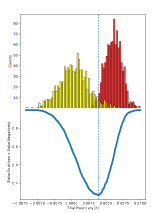
\includegraphics[width=\textwidth, trim={0 0 0 1cm}, clip]{Immagini/Es7Fig3.pdf}
	\label{Es7Fig3}
\end{figure}

\begin{lstlisting}[language=python, style=Pystyle, caption=\texttt{Python} code for Fisher's boundary value optimization, label=listing:tcut]
[...]
## Significance and Specificity optimization and consequent t_cut determination

t=np.concatenate((x11,x00),axis=0)  ## Definition of Fisher Statistic
q=np.linspace(min(t),max(t),len(t)) ## Homogeneuous domain for optimum-value search
alpha=np.zeros(len(t))              ## alpha := 1 - E_1 -> #{False Negatives}
beta=np.zeros(len(t))               ## beta  := E_0 -----> #{False Positives}

for i in range(0,len(q)):
	alpha[i]=(x11<q[i]).sum()/n1 ## Rejection of H1 when H1 is true
	beta[i]=(x00>q[i]).sum()/n0  ## Acceptance of H1 when H1 is false

ToMinimize=alpha+beta
best=min(ToMinimize)

t_cut=np.mean(q[ToMinimize==best]) ## There can be more than one best-match...
print (round(t_cut,6) , ': t_cut optimum value')

plt.axvline(t_cut) 
plt.xlabel('Projected Data')
plt.ylabel('Counts')

## Plotting alpha+beta as a function of trial t_cut (i.e. q)

plt.figure('Minimization Functional')
plt.plot(q,ToMinimize, linewidth = 5)
plt.xlabel('Trial Boundary [t]')
plt.ylabel('(False Positives + False Negatives)')
plt.axvline(np.mean(q[ToMinimize==best]))
plt.show()

## Identified signal purity computation

optalpha=np.mean(alpha[np.where(((q-t)**2)**0.5==np.min((q-t)**2)**0.5)])
optbeta=np.mean(beta[np.where(((q-t)**2)**0.5==np.min((q-t)**2)**0.5)])

print(round(optalpha,6), ': alpha optimum value')
print(round(optbeta,6), ': beta optimum value')
print(round(1-optalpha,6)/(round(optbeta,6)+round(1-optalpha,6)), ': Signal Purity')
\end{lstlisting}

\newpage

\noindent Infine è stata eseguita un'analisi della curva ROC  (\emph{Receiver Operating Characteristic}), la cui area sottesa (AUC) fornisce informazioni sulla qualità del test d'ipotesi implementato: più l'integrale dell'efficienza di segnale valutato come funzione dell'efficienza di fondo (= 1 - rigezione del fondo) è prossimo all'unità e più il test d'ipotesi garantisce di ottenere un segnale ricostruito di grande purezza. Nel nostro caso l'accuratezza con cui è stato approssimato l'integrale (Cfr. Listato~\ref{Es7ROClist}) non è stata sufficiente a risolvere la differenza $\mathop{\delta A} = (1-\mathrm{AUC})$, decisamente piccola come evidente in Figura~\ref{Es7ROCfig}.

\begin{figure}
	\centering
	\includegraphics[width=.7\textwidth]{Immagini/Es7Fig4.pdf}
	\caption{\emph{Receiver Operating Characteristic Analysis for Fisher test} }
	\label{Es7ROCfig}
\end{figure}

\begin{lstlisting}[language=python, style=Pystyle, caption=\texttt{Python} code for ROC curve analysis for Fisher test , label=Es7ROClist]
[...]
## ROC curve determination

plt.figure('ROC curve')
plt.plot(beta,1-alpha, linewidth = 5, color='green')
plt.xlabel('False Positive Rate [Background Efficiency]')
plt.ylabel('True Positive Rate [Signal Efficiency]')
plt.title('ROC curve')
plt.show()

## Area under the ROC curve (Integrating in [0,1] with "trapezoid-rule")

SamplingPts = beta.shape[0]
I = 0.5*alpha[0] + 0.5*alpha[beta.shape[0]-1]
for j in range(1,SamplingPts):
	I += alpha[j]
	dx = beta[j] - beta[j-1]
	I *= dx
I += 1

print('ROC area: ', I)
\end{lstlisting}